% Provenance (never printed): cycle 4 SVT, "La planete Terre": the history of
% the Earth read in the rocks, relative dating (superposition, recoupement,
% inclusion, continuite paleontologique), the ages of the Earth, eras and
% periods, the scale of geological time; see sources/book1/PROVENANCE.md.
% Book 1, grade 7, chapter 5.
% Vocabulary guard: owns relative dating / absolute age, the four principles,
% unconformity, era and geological period, the geological time scale. The
% method of radiometric dating is the physics books' and grade 12's: told
% here in two sentences, never defined. Fossils as evidence of evolution are
% the biology books' (one sentence of prose). "Ice age" is grade 8's: not used.
\chapter{أعمار الأرض}\label{ch:g7:geological-time}

في يونيو 1788، زار الجيولوجي الأسكتلندي جيمس هاتون وصديقان له، هما
الرياضي جون بلايفير والكيميائي جيمس هول، رأس سيكار بوينت، وهو رأس صخري
«جرّده \omterm{def:g2:water-on-earth:ocean}{البحر}» على \omterm{def:g1:landscapes-around-us:water}{ساحل} أسكتلندا. وفي أسفل \omterm{def:g3:stones-pebbles-sand:rock}{الصخر} رأوا طبقات رمادية منتصبة
على حافتها، شبه رأسية. وفوقها استلقت طبقات من الحجر الرملي الأحمر، مائلة
ميلًا خفيفًا. وشرح هاتون ما حدث: فالطبقات الرمادية وُضعت مستوية في قاع
\omterm{def:g2:water-on-earth:ocean}{بحر}، ثم دُفعت حتى انتصبت، ثم تآكلت، قبل أن يوضع \omterm{def:g3:stones-pebbles-sand:sand}{الرمل} الأحمر فوقها. وكل
خطوة من هذه الخطوات احتاجت إلى زمن هائل. وكتب بلايفير لاحقًا: «لقد بدا
العقل وكأنه يُصاب بالدوار من النظر بعيدًا إلى هذا الحد في هاوية الزمن.»
% ledger: ncse:siccar-point

\begin{omfigure}
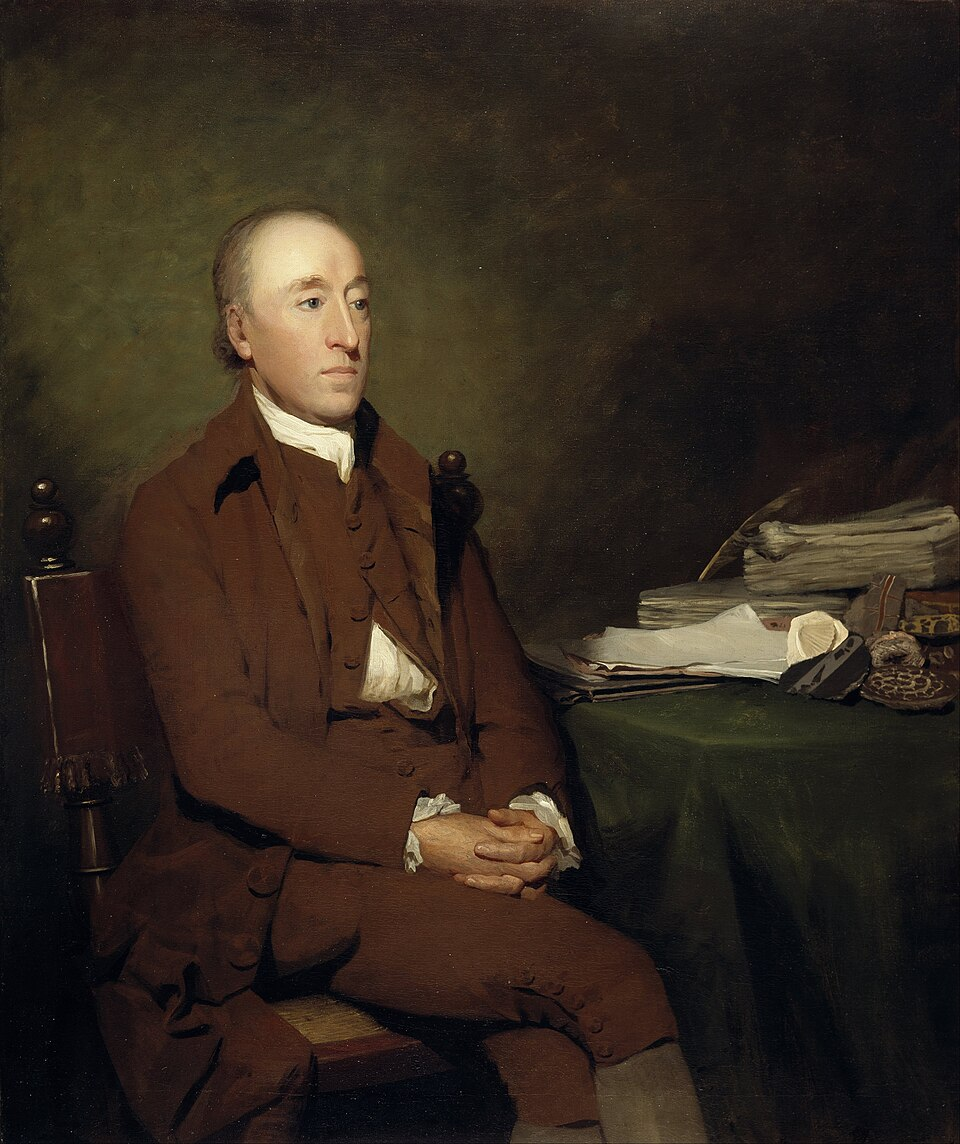
\includegraphics[width=0.3\linewidth]{images/book1/g7-hutton.jpg}

{\small جيمس هاتون (1726--1797)، بريشة هنري ريبورن. رأى هاتون في كل
طبقة مدة من الزمن، أقدمها في الأسفل حيثما لم تنقلب الطبقات. اللوحة ملك
عام، عبر ويكيميديا كومنز.}
% ledger: commons:hutton-portrait, usgs:hutton-smith
\label{fig:g7:geological-time:hutton}
\end{omfigure}

كيف نعرف أي الصخرين أقدم من الآخر، دون أي تاريخ مكتوب عليه؟ وكم عمر
الأرض؟ وكيف يمكن أصلًا أن نتصور تاريخًا بهذا الطول؟

\begin{recall}
تترسب \omterm{def:g7:sediments-and-fossils:sediment}{الرواسب} في طبقات، بعضها فوق بعض، وتتصلب فتصير \omterm{def:g3:stones-pebbles-sand:rock}{صخرًا} رسوبيًا؛ \omterm{def:g7:sediments-and-fossils:fossil}{والأحافير}
بقايا كائنات حية أو آثارها محفوظة في \omterm{def:g3:stones-pebbles-sand:rock}{الصخر} (\cref{ch:g7:sediments-and-fossils}).
و\emph{\omterm{def:g7:earthquakes:fault}{الصدع}} كسر في \omterm{def:g3:stones-pebbles-sand:rock}{الصخور} تحرك على طوله الجانبان
(\cref{ch:g7:earthquakes}). والغرانيت \emph{\omterm{def:g6:rocks-and-minerals:rock-families}{صخر ناري}}: يتكون حين يبرد \omterm{def:g3:stones-pebbles-sand:rock}{صخر}
منصهر ببطء، في أعماق باطن الأرض؛ والشست \emph{\omterm{def:g6:rocks-and-minerals:rock-families}{صخر متحول}}، غيّرته الحرارة
والضغط؛ والرصيص \omterm{def:g6:rocks-and-minerals:rock-families}{صخر رسوبي} مكوَّن من \omterm{def:g3:stones-pebbles-sand:pebble}{حصى} ملتحمة بعضها ببعض
(\cref{ch:g6:rocks-and-minerals}).
\end{recall}

\section{أيهما جاء أولًا؟}

يستطيع المؤرخون أن يرتبوا الأحداث حتى دون تواريخها. فالحرب العالمية الأولى
جاءت قبل الثانية: اسماهما يقولان ذلك. ولم يكن التلفزيون قد دخل البيوت بعد
حين طار الأخوان رايت أول مرة عام 1903، لكن كثيرين شاهدوا أولى الخطوات على
القمر عبر التلفزيون عام 1969: فالطيران جاء أولًا، ثم التلفزيون في البيوت،
ثم القمر. فجمع الأدلة ومقارنتها يكفيان لمعرفة الترتيب. ولا يوجد لمعظم
تاريخ الأرض أي سجل مكتوب على الإطلاق، والجيولوجيون يعملون بالطريقة نفسها:
فهم يستعملون أدلة محفوظة في \omterm{def:g3:stones-pebbles-sand:rock}{الصخور}.
% ledger: usgs:events-order

\begin{definition}[التأريخ النسبي والعمر المطلق]\label{def:g7:geological-time:relative-dating}
\emph{التأريخ النسبي}\index{تأريخ نسبي} يرتب \omterm{def:g3:stones-pebbles-sand:rock}{الصخور} والأحداث، من الأقدم
إلى الأحدث، دون أن يقول منذ كم سنة وقعت: هذا \omterm{def:g3:stones-pebbles-sand:rock}{الصخر} أقدم من ذاك.
و\emph{العمر المطلق}\index{عمر مطلق} عمر يُعطى بعدد من السنين، مثل
«\num{300} مليون سنة».
\end{definition}

\section{أربعة مبادئ لترتيب الصخور}

أربعة مبادئ بسيطة تؤدي معظم عمل \omterm{def:g7:geological-time:relative-dating}{التأريخ النسبي}. وهي مصوَّرة أدناه، في أربعة
أجراف متخيَّلة. وقد صاغ أولها نيكولاس ستينو عام 1669؛ وبنى عليه هاتون في
أواخر القرن الثامن عشر.
% ledger: usgs:hutton-smith, og:stratigraphy-principles

\begin{omfigure}
\tikzset{
  trilo/.pic={\fill[black!65] (0,0) ellipse (0.13 and 0.085);
              \draw[white, line width=0.3pt] (-0.11,0.028) -- (0.11,0.028) (-0.11,-0.028) -- (0.11,-0.028);},
  ammo/.pic={\draw[black!75, line width=0.45pt] (0,0) circle (0.1) (0,0) circle (0.062) (0,0) circle (0.028);}
}
\begin{minipage}[t]{0.49\linewidth}\centering
\begin{tikzpicture}[font=\footnotesize]
  \fill[lith sandstone] (0,0) rectangle (4.4,0.6);
  \fill[lith shale] (0,0.6) rectangle (4.4,1.2);
  \fill[lith limestone] (0,1.2) rectangle (4.4,1.8);
  \fill[lith sandstone] (0,1.8) rectangle (4.4,2.4);
  \foreach \k in {1,2,3,4} \node[fill=white, inner sep=1pt] at (0.35,0.6*\k-0.3) {\k};
  \draw (0,0) rectangle (4.4,2.4);
  \foreach \y in {0.6,1.2,1.8} \draw[contact] (0,\y) -- (4.4,\y);
  \draw[-{Stealth}, line width=0.8pt] (4.75,0.1) -- (4.75,2.3);
  \node[anchor=west] at (4.85,2.2) {الأحدث};
  \node[anchor=west] at (4.85,0.2) {الأقدم};
\end{tikzpicture}

{\small (أ) التراكب: الطبقة 1 تكونت أولًا، والطبقة 4 أخيرًا.}
\end{minipage}\hfill
\begin{minipage}[t]{0.49\linewidth}\centering
\begin{tikzpicture}[font=\footnotesize]
  % left block, below the fault
  \begin{scope}
    \clip (0,0) -- (3.75,0) -- (3.25,2.4) -- (0,2.4) -- cycle;
    \fill[lith sandstone] (0,0) rectangle (5,0.6);
    \fill[lith shale] (0,0.6) rectangle (5,1.2);
    \fill[lith limestone] (0,1.2) rectangle (5,1.8);
    \fill[lith granite] (1.2,0) -- (1.85,0) -- (1.75,0.9) -- (1.9,1.8) -- (1.15,1.8) -- (1.3,0.9) -- cycle;
    \fill[lith sandstone] (0,1.8) rectangle (5,2.4);
    \foreach \y in {0.6,1.2} {\draw[contact] (0,\y) -- (1.25,\y); \draw[contact] (1.8,\y) -- (5,\y);}
    \draw[contact] (1.2,0) -- (1.3,0.9) -- (1.15,1.8) (1.85,0) -- (1.75,0.9) -- (1.9,1.8);
    \draw[contact] (0,1.8) -- (5,1.8);
  \end{scope}
  % right block, moved down along the fault
  \begin{scope}
    \clip (3.75,0) -- (5,0) -- (5,2.05) -- (3.32,2.05) -- cycle;
    \fill[lith sandstone] (3,-0.35) rectangle (5,0.25);
    \fill[lith shale] (3,0.25) rectangle (5,0.85);
    \fill[lith limestone] (3,0.85) rectangle (5,1.45);
    \fill[lith sandstone] (3,1.45) rectangle (5,2.05);
    \foreach \y in {0.25,0.85,1.45} \draw[contact] (3,\y) -- (5,\y);
  \end{scope}
  \draw (0,0) -- (5,0) -- (5,2.05) -- (3.32,2.05) (3.25,2.4) -- (0,2.4) -- (0,0);
  \draw[fault] (3.75,0) -- (3.25,2.4);
  \node[anchor=south, fill=white, inner sep=1pt] at (1.5,2.45) {الغرانيت};
  \draw[black!70] (1.5,2.45) -- (1.52,1.6);
  \node[anchor=south] at (4.2,2.45) {الصدع};
  \draw[black!70] (4.0,2.45) -- (3.4,1.75);
\end{tikzpicture}

{\small (ب) التقاطع: الغرانيت أحدث من الطبقات الثلاث التي يقطعها، وأقدم من
الطبقة العليا؛ \omterm{def:g7:earthquakes:fault}{والصدع}، الذي يكسرها كلها، هو الأحدث.}
\end{minipage}

\bigskip
\begin{minipage}[t]{0.49\linewidth}\centering
\begin{tikzpicture}[font=\footnotesize]
  \fill[lith granite] (0,0) -- (4.4,0) -- (4.4,1.05) .. controls (3.4,0.95) and (2.6,1.2) .. (1.6,1.0) .. controls (0.9,0.88) and (0.4,1.1) .. (0,1.0) -- cycle;
  \fill[lith conglomerate] (0,2.4) -- (4.4,2.4) -- (4.4,1.05) .. controls (3.4,0.95) and (2.6,1.2) .. (1.6,1.0) .. controls (0.9,0.88) and (0.4,1.1) .. (0,1.0) -- cycle;
  \foreach \x/\y/\a/\b in {0.5/1.35/0.2/0.12, 1.3/1.25/0.16/0.1, 2.1/1.45/0.22/0.13, 2.9/1.3/0.17/0.11, 3.7/1.4/0.2/0.12, 0.9/1.8/0.15/0.1, 2.5/1.95/0.17/0.1, 3.4/1.85/0.14/0.09}
    \filldraw[fill=omLithGranite, draw=black!70, line width=0.3pt] (\x,\y) ellipse [x radius=\a, y radius=\b];
  \draw[unconformity] (0,1.0) .. controls (0.4,1.1) and (0.9,0.88) .. (1.6,1.0) .. controls (2.6,1.2) and (3.4,0.95) .. (4.4,1.05);
  \draw (0,0) rectangle (4.4,2.4);
  \node[fill=white, inner sep=1pt] at (2.2,0.45) {الغرانيت};
  \node[anchor=west] at (4.5,1.7) {الرصيص};
  \node[anchor=west, align=left] at (4.5,1.15) {حصى من\\الغرانيت};
  \draw[black!70] (4.5,1.15) -- (3.85,1.4);
\end{tikzpicture}

{\small (ج) الاحتواء: \omterm{def:g3:stones-pebbles-sand:pebble}{حصى} الغرانيت أقدم من الرصيص الذي
يحتويها.}
\end{minipage}\hfill
\begin{minipage}[t]{0.49\linewidth}\centering
\begin{tikzpicture}[font=\footnotesize]
  % place A
  \fill[lith shale] (0,0) rectangle (1.3,0.8);
  \fill[lith limestone] (0,0.8) rectangle (1.3,1.6);
  \fill[lith sandstone] (0,1.6) rectangle (1.3,2.4);
  \draw (0,0) rectangle (1.3,2.4); \draw[contact] (0,0.8) -- (1.3,0.8) (0,1.6) -- (1.3,1.6);
  \foreach \x in {0.3,0.65,1.0} {\pic at (\x,0.4) {trilo}; \pic at (\x,1.2) {ammo};}
  \node[anchor=south] at (0.65,2.45) {\foreignlanguage{arabic}{المكان A}};
  % place B
  \fill[lith sandstone] (3.6,0.4) rectangle (4.9,1.0);
  \fill[lith shale] (3.6,1.0) rectangle (4.9,2.0);
  \fill[lith limestone] (3.6,0) rectangle (4.9,0.4);
  \draw (3.6,0) rectangle (4.9,2.0); \draw[contact] (3.6,0.4) -- (4.9,0.4) (3.6,1.0) -- (4.9,1.0);
  \foreach \x in {3.9,4.25,4.6} {\pic at (\x,0.7) {trilo}; \pic at (\x,1.5) {ammo};}
  \node[anchor=south] at (4.25,2.45) {\foreignlanguage{arabic}{المكان B}};
  \draw[dashed, black!70] (1.3,0.8) -- (3.6,1.0) (1.3,0) -- (3.6,0.4) (1.3,1.6) -- (3.6,2.0);
  \pic at (2.15,-0.3) {trilo}; \node[anchor=west] at (2.3,-0.3) {ثلاثي فصوص};
  \pic at (2.15,2.3) {ammo}; \node[anchor=west] at (2.3,2.3) {أمونيت};
\end{tikzpicture}

{\small (د) التتابع الأحفوري: الطبقات التي فيها \omterm{def:g7:sediments-and-fossils:fossil}{الأحافير} نفسها من العمر
نفسه، وإن اختلفت صخورها.}
\end{minipage}

\medskip
{\small مبادئ \omterm{def:g7:geological-time:relative-dating}{التأريخ النسبي} الأربعة، في أربعة أجراف
متخيَّلة.}
% ledger: usgs:hutton-smith, usgs:cross-cutting, nps:cross-cutting, eli:relative-dating, usgs:fossil-succession
\label{fig:g7:geological-time:principles}
\end{omfigure}

\begin{definition}[مبدأ التراكب]\label{def:g7:geological-time:superposition}
\emph{مبدأ التراكب}\index{مبدأ التراكب}: في كومة من الطبقات الرسوبية لم
تنقلب، كل طبقة أحدث من الطبقة التي تحتها وأقدم من الطبقة التي فوقها.
فأقدم طبقة في الأسفل، وأحدثها في الأعلى.
\end{definition}
% ledger: usgs:hutton-smith, eli:relative-dating

\begin{definition}[مبدأ التقاطع]\label{def:g7:geological-time:cross-cutting}
\emph{مبدأ التقاطع}\index{مبدأ التقاطع}: \omterm{def:g3:stones-pebbles-sand:rock}{الصخر} أو البنية التي تقطع صخورًا
أخرى أحدث من \omterm{def:g3:stones-pebbles-sand:rock}{الصخور} التي تقطعها. فكتلة الغرانيت التي تخترق طبقات، \omterm{def:g7:earthquakes:fault}{والصدع}
الذي يكسرها، وسطح \omterm{def:g5:water-shapes-the-land:erosion}{التعرية} الذي يبريها، كلها أحدث من تلك الطبقات.
\end{definition}
% ledger: usgs:cross-cutting, nps:cross-cutting, eli:relative-dating

\begin{definition}[مبدأ الاحتواء]\label{def:g7:geological-time:inclusion}
\emph{مبدأ الاحتواء}\index{مبدأ الاحتواء}: قطع \omterm{def:g3:stones-pebbles-sand:rock}{صخر} ما الموجودة داخل \omterm{def:g3:stones-pebbles-sand:rock}{صخر}
آخر أقدم من \omterm{def:g3:stones-pebbles-sand:rock}{الصخر} الذي يحتويها. \omterm{def:g3:stones-pebbles-sand:pebble}{فحصى} الرصيص كانت موجودة قبل أن يتكون
الرصيص حولها.
\end{definition}
% ledger: eli:relative-dating

\begin{definition}[مبدأ التتابع الأحفوري]\label{def:g7:geological-time:fossil-succession}
\emph{مبدأ التتابع الأحفوري}\index{مبدأ التتابع الأحفوري}: أنواع الحيوانات
والنباتات التي توجد \omterm{def:g7:sediments-and-fossils:fossil}{أحافير} تتغير من الطبقات الأقدم إلى الأحدث، دائمًا
بالترتيب نفسه. \omterm{def:g3:stones-pebbles-sand:rock}{والصخور} التي تحوي الأنواع نفسها من \omterm{def:g7:sediments-and-fossils:fossil}{الأحافير} من العمر نفسه،
حتى حين تكون متباعدة.
\end{definition}
% ledger: usgs:fossil-succession


لا يصح \omterm{def:g7:geological-time:superposition}{مبدأ التراكب} إلا في الطبقات التي لم تنقلب: ففي أماكن قليلة، طوى
بناء \omterm{def:g1:landscapes-around-us:landform}{الجبال} كومة من الطبقات طيًّا شديدًا حتى صارت مقلوبة. وعندئذ يبحث
الجيولوجيون عن أدلة تبين في أي اتجاه تكونت الطبقات --- فآثار الأقدام
وعلامات التموج، مثلًا، تكون على السطح العلوي للطبقة. \omterm{def:g7:geological-time:fossil-succession}{ومبدأ التتابع
الأحفوري} يصح لأن الحياة على الأرض تغيرت عبر الزمن: فمعظم \omterm{def:g7:sediments-and-fossils:fossil}{الأحافير} تنتمي
إلى أنواع لم تعد تعيش في أي مكان. أما لماذا تغيرت الحياة، فتحكيه كتب
علم الأحياء.
% ledger: eli:relative-dating, usgs:fossil-succession, nps:ripple-marks

\begin{history}[وليام سميث، باني القنوات]
بين 1785 و1800، بينما كان هاتون يعمل في أسكتلندا، كان وليام سميث، وهو
مهندس إنجليزي يبني القنوات، يجمع الأصداف الأحفورية من الأحجار الجيرية
والسجّيل التي كان يحفر عبرها. فوجد أن كل طبقة تحوي أحافيرها الخاصة،
المختلفة عن \omterm{def:g7:sediments-and-fossils:fossil}{أحافير} الطبقات التي فوقها وتحتها. وباستعمال هذه \omterm{def:g7:sediments-and-fossils:fossil}{الأحافير}
علامات، استطاع أن يتعرف على الطبقة نفسها حيثما ظهرت، ورسم بعضًا من أولى
الخرائط الجيولوجية لمناطق واسعة.
\end{history}
% ledger: usgs:hutton-smith

\section{فجوات في السجل}

في سيكار بوينت، لم تتكون الطبقات الرمادية والحجر الرملي الأحمر واحدًا بعد
الآخر. فبينهما، مالت الطبقات الرمادية وارتفعت، ثم تآكلت زمنًا طويلًا
جدًا، ولم تُحفظ أي طبقة من ذلك الزمن. والسطح بين مجموعتي \omterm{def:g3:stones-pebbles-sand:rock}{الصخور} فجوة في
السجل.

\begin{definition}[عدم التوافق]\label{def:g7:geological-time:unconformity}
\emph{عدم التوافق}\index{عدم توافق} سطح \omterm{def:g5:water-shapes-the-land:erosion}{تعرية} بين مجموعتين من \omterm{def:g3:stones-pebbles-sand:rock}{الصخور}
تكونتا في زمنين متباعدين جدًا: \omterm{def:g3:stones-pebbles-sand:rock}{فالصخور} الأقدم تآكلت قبل أن توضع الأحدث
فوقها. وهو يدل على زمن طويل لم تُحفظ منه أي طبقة.
\end{definition}
% ledger: ncse:siccar-point, eli:relative-dating

\begin{omfigure}
\begin{tikzpicture}[font=\footnotesize, x=1cm, y=1cm]
  \def\stripes#1#2#3{% x0, width, top: vertical layers
    \foreach \i in {0,...,7} {
      \pgfmathsetmacro{\xa}{#1+\i*#2/8}
      \pgfmathsetmacro{\xb}{#1+(\i+1)*#2/8}
      \ifodd\i\def\lithc{omLithSchist}\else\def\lithc{omLithShale}\fi
      \fill[\lithc] (\xa,0) rectangle (\xb,#3);
      \draw[black!55, line width=0.3pt] (\xa,0) -- (\xa,#3);
    }}
  % 1: flat layers under the sea
  \fill[omSea!70] (0,1.6) rectangle (3.4,2.4);
  \foreach \k in {0,...,3} {
    \ifodd\k\def\lithc{omLithSchist}\else\def\lithc{omLithShale}\fi
    \fill[\lithc] (0,0.4*\k) rectangle (3.4,0.4*\k+0.4);
    \draw[black!55, line width=0.3pt] (0,0.4*\k) -- (3.4,0.4*\k);
  }
  \draw (0,0) rectangle (3.4,2.4);
  \node[anchor=north, align=center] at (1.7,-0.1) {\foreignlanguage{arabic}{1. طبقات توضع}\\مستوية في بحر};
  % 2: pushed up on end
  \begin{scope}[xshift=3.9cm]
    \begin{scope}
      \clip (0,0) -- (3.4,0) -- (3.4,1.7) -- (2.6,2.2) -- (1.6,1.75) -- (0.9,2.3) -- (0,1.8) -- cycle;
      \stripes{0}{3.4}{2.4}
    \end{scope}
    \draw (0,1.8) -- (0.9,2.3) -- (1.6,1.75) -- (2.6,2.2) -- (3.4,1.7);
    \draw (0,1.8) -- (0,0) -- (3.4,0) -- (3.4,1.7);
    \node[anchor=north, align=center] at (1.7,-0.1) {\foreignlanguage{arabic}{2. تُدفع حتى تنتصب}\\وترتفع فوق البحر};
  \end{scope}
  % 3: worn flat
  \begin{scope}[xshift=7.8cm]
    \stripes{0}{3.4}{1.3}
    \draw[unconformity] (0,1.3) -- (3.4,1.3);
    \draw (0,1.3) -- (0,0) -- (3.4,0) -- (3.4,1.3);
    \node[anchor=north, align=center] at (1.7,-0.1) {\foreignlanguage{arabic}{3. تتآكل}\\زمنًا طويلًا};
  \end{scope}
  % 4: new layers on top
  \begin{scope}[xshift=11.7cm]
    \stripes{0}{3.4}{1.3}
    \fill[om lith={red!22}{om sand}] (0,1.3) rectangle (3.4,1.85);
    \fill[om lith={red!30}{om sand}] (0,1.85) rectangle (3.4,2.4);
    \draw[contact] (0,1.85) -- (3.4,1.85);
    \draw[unconformity, line width=0.9pt] (0,1.3) -- (3.4,1.3);
    \draw (0,0) rectangle (3.4,2.4);
    \node[anchor=north, align=center] at (1.7,-0.1) {\foreignlanguage{arabic}{4. طبقات جديدة فوقها}\\إنه عدم توافق};
  \end{scope}
  \foreach \x in {3.45,7.35,11.25} \draw[-{Stealth}, line width=0.7pt] (\x,1.2) -- (\x+0.4,1.2);
\end{tikzpicture}

{\small كيف يتكون \omterm{def:g7:geological-time:unconformity}{عدم توافق} مثل الذي في سيكار بوينت. والخط المتموج هو \omterm{def:g7:geological-time:unconformity}{عدم
التوافق}: فالزمن الطويل للمرحلتين 2 و3 لم يترك وراءه أي طبقة.}
% ledger: ncse:siccar-point
\label{fig:g7:geological-time:unconformity}
\end{omfigure}

\section{قراءة تاريخ منطقة}

المقطع الجيولوجي يُظهر \omterm{def:g3:stones-pebbles-sand:rock}{الصخور} كما تبدو في قطع رأسي في الأرض. والمبادئ
الأربعة تحوّله إلى قصة.

\begin{method}[ترتيب أحداث مقطع]\label{met:g7:geological-time:ordering}
\begin{enumerate}
  \item ابحث عن أقدم \omterm{def:g3:stones-pebbles-sand:rock}{الصخور}: تلك التي يقطعها كل ما عداها، أو تقع في أسفل
        الكومة.
  \item ابحث عن كل \omterm{def:g3:stones-pebbles-sand:rock}{صخر} أو بنية تقطع غيرها (غرانيت، أو \omterm{def:g7:earthquakes:fault}{صدع}، أو سطح \omterm{def:g5:water-shapes-the-land:erosion}{تعرية}):
        فهي أحدث من كل ما تقطعه.
  \item اقرأ الطبقات من الأسفل إلى الأعلى (التراكب)، وابحث عن حالات \omterm{def:g7:geological-time:unconformity}{عدم
        التوافق}، حيث يغيب الزمن.
  \item الطبقات توضع مستوية: فإن كانت مائلة أو مطوية، فالطي جاء بعدها.
  \item اكتب الأحداث بالترتيب، من الأقدم إلى الأحدث، مع دليل كل حدث.
\end{enumerate}
\end{method}
% ledger: eli:relative-dating, usgs:cross-cutting, nps:cross-cutting

\begin{omfigure}
\begin{tikzpicture}
\begin{axis}[x=1.4cm, y=0.007cm, xmin=0, xmax=10, ymin=-500, ymax=300,
  axis on top, tick label style={font=\scriptsize}, label style={font=\small},
  xlabel={المسافة شرقًا من النقطة E بالكيلومترات}, ylabel={الارتفاع بالأمتار},
  ytick={-400,-200,0,200}, clip mode=individual]
\addplot[lith schist, draw=black, line width=0.3pt, even odd rule] table {figdata/out/grade-7-varden_history-unit-schist.dat};
\addplot[lith granite, draw=black, line width=0.3pt, even odd rule] table {figdata/out/grade-7-varden_history-unit-granite.dat};
\addplot[om lith={icsTriassic!35}{om sand}, draw=black, line width=0.3pt, even odd rule] table {figdata/out/grade-7-varden_history-unit-sandstone.dat};
\addplot[om lith={icsJurassic!40}{om limestone}, draw=black, line width=0.3pt, even odd rule] table {figdata/out/grade-7-varden_history-unit-limestone.dat};
\addplot[om lith={icsJurassic!15}{om shale}, draw=black, line width=0.3pt, even odd rule] table {figdata/out/grade-7-varden_history-unit-shale.dat};
\addplot[om lith={icsCretaceous!35}{om limestone}, draw=black, line width=0.3pt, even odd rule] table {figdata/out/grade-7-varden_history-unit-chalk.dat};
\addplot[lith alluvium, draw=black, line width=0.3pt, even odd rule] table {figdata/out/grade-7-varden_history-unit-alluvium.dat};
\addplot[omThm, line width=1.3pt] table {figdata/out/grade-7-varden_history-base.dat};
\addplot[black, line width=0.8pt] table {figdata/out/grade-7-varden_history-ground.dat};
\addplot[fault, line width=1.3pt] table {figdata/out/grade-7-varden_history-fault.dat};
\node[font=\small, above right] at (axis cs:0,300) {\foreignlanguage{arabic}{E في الغرب}};
\node[font=\small, above left] at (axis cs:10,300) {\foreignlanguage{arabic}{F في الشرق}};
\end{axis}
\end{tikzpicture}

\smallskip
{\small\setlength{\tabcolsep}{4pt}
\begin{tabular}{@{}llll@{}}
\tikz\fill[lith schist, draw=black] (0,0) rectangle (0.5,0.3); الشست &
\tikz\fill[lith granite, draw=black] (0,0) rectangle (0.5,0.3); الغرانيت &
\tikz\fill[om lith={icsTriassic!35}{om sand}, draw=black] (0,0) rectangle (0.5,0.3); الحجر الرملي &
\tikz\fill[om lith={icsJurassic!40}{om limestone}, draw=black] (0,0) rectangle (0.5,0.3); الحجر الجيري \\
\tikz\fill[om lith={icsJurassic!15}{om shale}, draw=black] (0,0) rectangle (0.5,0.3); السجّيل &
\tikz\fill[om lith={icsCretaceous!35}{om limestone}, draw=black] (0,0) rectangle (0.5,0.3); الطباشير &
\tikz\fill[lith alluvium, draw=black] (0,0) rectangle (0.5,0.3); \omterm{def:g3:stones-pebbles-sand:sand}{رمل} \omterm{def:g1:landscapes-around-us:water}{النهر} &
\tikz\draw[omThm, line width=1.3pt] (0,0.15) -- (0.5,0.15); قاعدة الحجر الرملي \\
\end{tabular}}

\smallskip
{\small المقطع E--F، من الغرب (E) إلى الشرق (F) عبر وسط تلال فاردن،
المنطقة المتخيَّلة في هذه السلسلة، مرورًا بغرانيتها. والخط الأسود السميك
هو \omterm{def:g7:earthquakes:fault}{الصدع}. والارتفاعات ممطوطة 5 مرات مقارنة بالمسافات، لتسهل رؤية
الطبقات.}
% ledger: (invented region: figdata/shared/region.py, section E--F by figdata/grade-7/varden_history.py)
\label{fig:g7:geological-time:section}
\end{omfigure}

\begin{example}[تاريخ تلال فاردن]\label{ex:g7:geological-time:varden}
طبّق الطريقة على المقطع E--F.
\begin{enumerate}
  \item الشست يقطعه الغرانيت ويقع تحت كل الطبقات: إنه أقدم \omterm{def:g3:stones-pebbles-sand:rock}{صخر}.
  \item الغرانيت يقطع الشست (التقاطع)، فهو أحدث منه. ولا يقطع أيًّا من
        الطبقات التي فوقه: فهو أقدم من الحجر الرملي.
  \item برد الغرانيت في أعماق باطن الأرض، ومع ذلك فإن قاعدة الحجر الرملي،
        التي تستقر على الشست، تبلغ أعلى الغرانيت: \omterm{def:g3:stones-pebbles-sand:rock}{فالصخور} التي كانت
        تغطيهما تآكلت قبل مجيء \omterm{def:g3:stones-pebbles-sand:sand}{الرمل}. فقاعدة الحجر الرملي \omterm{def:g7:geological-time:unconformity}{عدم توافق}.
  \item الحجر الرملي والحجر الجيري والسجّيل والطباشير وُضعت بهذا الترتيب
        (التراكب).
  \item وُضعت الطبقات مستوية، لكنها اليوم مطوية، مقوَّسة إلى الأعلى فوق
        الغرانيت ومنحنية إلى الأسفل أبعد نحو الشرق: فالطي جاء بعد
        الطباشير.
  \item \omterm{def:g7:earthquakes:fault}{الصدع} يكسر كل الطبقات المطوية: فهو أحدث من الطي.
  \item سطح الأرض الحالي يقطع كل شيء، \omterm{def:g3:stones-pebbles-sand:sand}{ورمل} \omterm{def:g1:landscapes-around-us:water}{النهر} يستقر فوقه: \omterm{def:g5:water-shapes-the-land:erosion}{فالتعرية}
        \omterm{def:g1:landscapes-around-us:water}{والأنهار} هي أحدث الأحداث.
\end{enumerate}
التاريخ، الأقدم أولًا: الشست؛ الغرانيت؛ \omterm{def:g5:water-shapes-the-land:erosion}{التعرية}؛ الطبقات الأربع؛ الطي؛
\omterm{def:g7:earthquakes:fault}{الصدع}؛ \omterm{def:g5:water-shapes-the-land:erosion}{تعرية} اليوم \omterm{def:g3:stones-pebbles-sand:sand}{ورمل} \omterm{def:g1:landscapes-around-us:water}{النهر}.
% ledger: (invented region: figdata/grade-7/varden_history.py main table)
\end{example}

\omterm{def:g7:geological-time:relative-dating}{التأريخ النسبي} يعطي ترتيب الأحداث، لا تواريخها ولا مدة كل منها: فالطريقة
تقول إن \omterm{def:g7:earthquakes:fault}{الصدع} أحدث من الطباشير، لكنها لا تقول بكم سنة.

\section{الحقب والعصور}

يتيح التتابع الأحفوري للجيولوجيين أن يطابقوا الطبقات في العالم كله. وبجمع
ملاحظاتهم، قسّموا تاريخ الأرض إلى مدد من الزمن، كما يتحدث المؤرخون عن
القرون وعن عهود الملوك.
% ledger: usgs:hutton-smith, usgs:fossil-succession

\begin{omfigure}
\begin{tikzpicture}[font=\footnotesize]
\begin{axis}[name=long, x dir=reverse, xmin=0, xmax=4600, ymin=0, ymax=1,
  width=14.3cm, height=1.7cm, scale only axis, axis y line=none, axis x line*=bottom,
  xtick={4500,4000,3000,2000,1000}, tick label style={font=\scriptsize}, clip=false]
  \pgfplotsinvokeforeach{Hadean,Archean,Proterozoic,Phanerozoic}{
    \addplot[fill=ics#1, draw=black!70, line width=0.3pt] table {figdata/out/grade-7-time_scale-bar-#1.dat};}
  \node[anchor=center, font=\scriptsize, fill=white, fill opacity=0.85, text opacity=1, inner sep=1pt] at (axis cs:4299,0.5) {الدهر الجهنمي};
  \node[anchor=center, font=\scriptsize, fill=white, fill opacity=0.85, text opacity=1, inner sep=1pt] at (axis cs:3265.5,0.5) {الدهر السحيق};
  \node[anchor=center, font=\scriptsize, fill=white, fill opacity=0.85, text opacity=1, inner sep=1pt] at (axis cs:1519.4,0.5) {دهر الحياة الطليعية};
  \node[anchor=center, font=\scriptsize, fill=white, fill opacity=0.85, text opacity=1, inner sep=1pt] at (axis cs:269.4,0.5) {الحياة الظاهرة};
  \coordinate (z1) at (axis cs:538.8,0);
  \coordinate (z2) at (axis cs:0,0);
\end{axis}
\begin{axis}[at={(long.south west)}, anchor=north west, yshift=-1.3cm,
  x dir=reverse, xmin=0, xmax=540, ymin=0, ymax=3.2,
  width=14.3cm, height=3.6cm, scale only axis, axis y line=none, axis x line*=bottom,
  xtick={500,400,300,200,100,0}, tick label style={font=\scriptsize},
  xlabel={ملايين السنين قبل اليوم}, label style={font=\small}, clip=false]
  \pgfplotsinvokeforeach{Paleozoic,Mesozoic,Cenozoic}{
    \addplot[fill=ics#1, draw=black!70, line width=0.3pt] table[x=age, y expr=2.4+0.8*\thisrow{y}] {figdata/out/grade-7-time_scale-bar-#1.dat};}
  \pgfplotsinvokeforeach{Cambrian,Ordovician,Silurian,Devonian,Carboniferous,Permian,Triassic,Jurassic,Cretaceous,Paleogene,Neogene,Quaternary}{
    \addplot[fill=ics#1, draw=black!70, line width=0.3pt] table[x=age, y expr=2.4*\thisrow{y}] {figdata/out/grade-7-time_scale-bar-#1.dat};}
  \node[anchor=center, font=\footnotesize\bfseries, fill=white, fill opacity=0.85, text opacity=1, inner sep=1pt] at (axis cs:395.351,2.8) {حقبة الحياة القديمة};
  \node[anchor=center, font=\footnotesize\bfseries, fill=white, fill opacity=0.85, text opacity=1, inner sep=1pt] at (axis cs:158.951,2.8) {حقبة الحياة الوسطى};
  \node[anchor=center, font=\footnotesize\bfseries, fill=white, fill opacity=0.85, text opacity=1, inner sep=1pt] at (axis cs:33,2.8) {حقبة الحياة الحديثة};
  \node[anchor=center, rotate=90, font=\scriptsize, fill=white, fill opacity=0.85, text opacity=1, inner sep=1pt] at (axis cs:512.825,1.2) {الكمبري};
  \node[anchor=center, rotate=90, font=\scriptsize, fill=white, fill opacity=0.85, text opacity=1, inner sep=1pt] at (axis cs:464.975,1.2) {الأوردوفيشي};
  \node[anchor=center, rotate=90, font=\scriptsize, fill=white, fill opacity=0.85, text opacity=1, inner sep=1pt] at (axis cs:431.36,1.2) {السيلوري};
  \node[anchor=center, rotate=90, font=\scriptsize, fill=white, fill opacity=0.85, text opacity=1, inner sep=1pt] at (axis cs:389.24,1.2) {الديفوني};
  \node[anchor=center, rotate=90, font=\scriptsize, fill=white, fill opacity=0.85, text opacity=1, inner sep=1pt] at (axis cs:328.88,1.2) {الكربوني};
  \node[anchor=center, rotate=90, font=\scriptsize, fill=white, fill opacity=0.85, text opacity=1, inner sep=1pt] at (axis cs:275.401,1.2) {البرمي};
  \node[anchor=center, rotate=90, font=\scriptsize, fill=white, fill opacity=0.85, text opacity=1, inner sep=1pt] at (axis cs:226.651,1.2) {الترياسي};
  \node[anchor=center, rotate=90, font=\scriptsize, fill=white, fill opacity=0.85, text opacity=1, inner sep=1pt] at (axis cs:172.25,1.2) {الجوراسي};
  \node[anchor=center, rotate=90, font=\scriptsize, fill=white, fill opacity=0.85, text opacity=1, inner sep=1pt] at (axis cs:104.55,1.2) {الطباشيري};
  \node[anchor=center, rotate=90, font=\scriptsize, fill=white, fill opacity=0.85, text opacity=1, inner sep=1pt] at (axis cs:44.52,1.2) {الباليوجيني};
  \node[anchor=center, rotate=90, font=\scriptsize, fill=white, fill opacity=0.85, text opacity=1, inner sep=1pt] at (axis cs:12.81,1.2) {النيوجيني};
  \node[anchor=west, xshift=3pt, font=\scriptsize] at (axis cs:1.29,1.2) {الرباعي};
  \coordinate (w1) at (axis cs:540,3.2);
  \coordinate (w2) at (axis cs:0,3.2);
\end{axis}
\draw[dashed, black!60] (z1) -- ++(0,-0.5) -- (w1) (z2) -- (w2);
\end{tikzpicture}

{\small \omterm{def:g7:geological-time:time-scale}{السلم الزمني الجيولوجي}، بألوان الجدول الدولي. في الأعلى: تاريخ الأرض
كله. وفي الأسفل: جزؤه الأخير، دهر الحياة الظاهرة، ممدودًا: حقبه الثلاث،
\omterm{def:g7:geological-time:era-period}{والعصور الجيولوجية} الاثنا عشر. والأعمار بملايين السنين قبل اليوم.}
% ledger: ics:base.Hadean, ics:base.Archean, ics:base.Proterozoic, ics:base.Paleozoic, ics:base.Mesozoic, ics:base.Cenozoic, ics:colour.Hadean (figdata/grade-7/time_scale.py reads every ics base and colour row of the shared ledger)
\label{fig:g7:geological-time:scale}
\end{omfigure}

\begin{definition}[الحقبة والعصر الجيولوجي]\label{def:g7:geological-time:era-period}
\emph{الحقبة}\index{حقبة} مدة طويلة من تاريخ الأرض، يحددها النوع العام
للحياة التي وُجدت في ذلك الزمن: حقبة الحياة القديمة، وحقبة الحياة الوسطى،
وحقبة الحياة الحديثة. وكل حقبة تنقسم إلى مدد أقصر، هي \emph{العصور
الجيولوجية}\index{عصر جيولوجي}، مثل العصر الجوراسي أو العصر الطباشيري.
\end{definition}
% ledger: usgs:hutton-smith

\begin{definition}[السلم الزمني الجيولوجي]\label{def:g7:geological-time:time-scale}
\emph{السلم الزمني الجيولوجي}\index{سلم زمني جيولوجي} هو قائمة أقسام
تاريخ الأرض مرتبة --- المدد الطويلة من تاريخها المبكر، \omterm{def:g7:geological-time:era-period}{والحقب}، \omterm{def:g7:geological-time:era-period}{والعصور
الجيولوجية} --- مع عمر بداية كل منها بالسنين. ويعطي جدول دولي كل قسم
اسمه وعمره ولونه.
\end{definition}
% ledger: ics:base.Hadean, ics:colour.Hadean


\omterm{def:g7:geological-time:era-period}{الحقب} الثلاث حديثة مقارنة بالتاريخ كله. فحقبة الحياة القديمة بدأت قبل
\num{538.8} مليون سنة، حين صارت \omterm{def:g7:sediments-and-fossils:fossil}{أحافير} الحيوانات ذات الأصداف شائعة؛ وحقبة
الحياة الوسطى امتدت من \num{251.9} إلى \num{66} مليون سنة مضت؛ وحقبة
الحياة الحديثة، \omterm{def:g7:geological-time:era-period}{الحقبة} التي نعيش فيها، بدأت قبل \num{66} مليون سنة. وقبل
حقبة الحياة القديمة تمتد ثلاث مدد طويلة، هي الدهر الجهنمي والدهر السحيق
ودهر الحياة الطليعية: وهي تغطي نحو 88~\% من تاريخ الأرض، لكن أحافيرها
نادرة. وعاشت الديناصورات في حقبة الحياة الوسطى: فقد سادت أكثر من
\num{100} مليون سنة، وبحلول نهاية العصر الطباشيري كانت قد اختفت كلها.
% ledger: ics:base.Paleozoic, ics:base.Mesozoic, ics:base.Cenozoic, usgs:numeric-scale, usgs:dinosaurs-extinct (figdata/grade-7/time_scale.py main table: 88.1 %)

تجد تلال فاردن مكانها على هذا السلم. فحجرها الرملي ترياسي، وحجرها الجيري
وسجّيلها جوراسيان، وطباشيرها طباشيري: والثلاثة كلها تنتمي إلى حقبة الحياة
الوسطى. وعلى المقطع E--F، رُسمت بدرجات باهتة من ألوان الجدول.
% ledger: (invented region: figdata/shared/region.py UNITS)

\section{تاريخ الأرض في سنة واحدة}

يصعب تصور الأعداد التي تُعد بمليارات السنين. فتخيّل بدلًا من ذلك تاريخ الأرض
كله مضغوطًا في سنة واحدة. تتكون الأرض في 1~يناير عند منتصف الليل؛ واليوم
هو دقة منتصف الليل في نهاية 31~ديسمبر. وعمر الأرض نحو \num{4540} مليون
سنة، فاليوم الواحد من هذه السنة يمثل $4540 \div 365$، أي نحو \num{12.4}
مليون سنة.
% ledger: usgs:age-earth (figdata/grade-7/earth_calendar.py)

\begin{omfigure}
\begin{tikzpicture}[font=\footnotesize]
\begin{axis}[xmin=0, xmax=365, ymin=0, ymax=1, width=15.2cm, height=0.9cm,
  scale only axis, axis y line=none, axis x line=none, clip=false]
  \addplot[ycomb, black!60, line width=0.4pt] table[x=day, y expr=1] {figdata/out/grade-7-earth_calendar-days.dat};
  \draw[black!70] (axis cs:0,0) rectangle (axis cs:365,1);
  \node[anchor=center, font=\scriptsize] at (axis cs:15.5,0.5) {يناير};
  \node[anchor=center, font=\scriptsize] at (axis cs:45,0.5) {فبراير};
  \node[anchor=center, font=\scriptsize] at (axis cs:74.5,0.5) {مارس};
  \node[anchor=center, font=\scriptsize] at (axis cs:105,0.5) {أبريل};
  \node[anchor=center, font=\scriptsize] at (axis cs:135.5,0.5) {مايو};
  \node[anchor=center, font=\scriptsize] at (axis cs:166,0.5) {يونيو};
  \node[anchor=center, font=\scriptsize] at (axis cs:196.5,0.5) {يوليو};
  \node[anchor=center, font=\scriptsize] at (axis cs:227.5,0.5) {أغسطس};
  \node[anchor=center, font=\scriptsize] at (axis cs:258,0.5) {سبتمبر};
  \node[anchor=center, font=\scriptsize] at (axis cs:288.5,0.5) {أكتوبر};
  \node[anchor=center, font=\scriptsize] at (axis cs:319,0.5) {نوفمبر};
  \node[anchor=center, font=\scriptsize] at (axis cs:349.5,0.5) {ديسمبر};
  \addplot[only marks, mark=triangle*, mark size=2.6pt, omThm, mark options={rotate=180}]
    table[x=day, y expr=1.18] {figdata/out/grade-7-earth_calendar.dat};
  \node[anchor=west, rotate=40, xshift=2pt, yshift=4pt, font=\scriptsize] at (axis cs:0,1.18) {\foreignlanguage{arabic}{1 يناير: تتكون الأرض}};
  \node[anchor=west, rotate=40, xshift=2pt, yshift=4pt, font=\scriptsize] at (axis cs:41,1.18) {\foreignlanguage{arabic}{11 فبراير: أقدم صخور عُثر عليها}};
  \node[anchor=west, rotate=40, xshift=2pt, yshift=4pt, font=\scriptsize] at (axis cs:83.61,1.18) {\foreignlanguage{arabic}{25 مارس: أقدم أحافير معروفة}};
  \node[anchor=east, rotate=-40, xshift=-2pt, yshift=4pt, font=\scriptsize] at (axis cs:321.68,1.18) {\foreignlanguage{arabic}{18 نوفمبر: الأصداف تصير شائعة}};
  \node[anchor=east, rotate=-40, xshift=-2pt, yshift=4pt, font=\scriptsize] at (axis cs:359.69,1.18) {\foreignlanguage{arabic}{26 ديسمبر: اختفت الديناصورات}};
\end{axis}
\end{tikzpicture}

{\small تاريخ الأرض في صورة سنة تقويمية واحدة: كل شهر يمثل نحو \num{373}
مليون سنة، وكل يوم نحو \num{12.4} مليون سنة. والتواريخ محسوبة من أعمار
الأحداث.}
% ledger: usgs:age-earth, usgs:oldest-rocks, usgs:numeric-scale, ics:base.Paleozoic, ics:base.Paleogene (figdata/grade-7/earth_calendar.py)
\label{fig:g7:geological-time:calendar}
\end{omfigure}

تصل أقدم \omterm{def:g3:stones-pebbles-sand:rock}{الصخور} التي عُثر عليها حتى الآن في 11~فبراير؛ وأقدم \omterm{def:g7:sediments-and-fossils:fossil}{الأحافير}
المعروفة في 25~مارس. وطوال معظم السنة، لا توجد حيوانات ذات أصداف، \omterm{def:g7:sediments-and-fossils:fossil}{والأحافير}
نادرة. ولا تصير الحيوانات ذات الأصداف شائعة إلا في 18~نوفمبر. أما
الديناصورات، فبعد أكثر من \num{100} مليون سنة من السيادة، تختفي في
26~ديسمبر، قبل نهاية السنة بخمسة أيام. ويصل نوعنا نحن في الساعة الأخيرة
من 31~ديسمبر: ومسألة هذا الفصل تبحث متى بالضبط.
% ledger: usgs:oldest-rocks, usgs:numeric-scale, ics:base.Paleozoic, ics:base.Paleogene, usgs:dinosaurs-extinct, hublin:jebel-irhoud

\begin{inthelab}[شريط الزمن]
داخل المبنى، افرد على أرض ممر \qty{4.54}{m} من شريط ورقي أو من لفافة ورق
آلة النقد: فبمعدل \qty{1}{mm} لكل مليون سنة، يتسع الشريط لتاريخ الأرض كله.
علّم بداية حقبة الحياة القديمة على بعد \qty{54}{cm} من النهاية، ونهاية
الديناصورات على بعد \qty{6.6}{cm} من النهاية. ثم حاول أن تعلّم تاريخ البشر
كله: فنوعنا، الذي يبلغ عمره نحو \num{300000} سنة، يملأ آخر \qty{0.3}{mm}،
وهي أرق من خط القلم.
\end{inthelab}
% ledger: usgs:age-earth, ics:base.Paleozoic, ics:base.Paleogene, hublin:jebel-irhoud

\section{الأعمار بالسنين}

لا يستطيع \omterm{def:g7:geological-time:relative-dating}{التأريخ النسبي} أن يقول منذ كم سنة تكوّن \omterm{def:g3:stones-pebbles-sand:rock}{صخر} ما. وقد صارت الأعمار
المطلقة ممكنة باكتشاف النشاط الإشعاعي. فبعض \omterm{def:g6:rocks-and-minerals:mineral}{المعادن} تحوي ذرات مشعة،
تتحول ببطء إلى ذرات أخرى بمعدل ثابت، هو نفسه في كل زمان ومكان؛ وقياس عدد
الذرات التي تحولت يعطي عمر \omterm{def:g6:rocks-and-minerals:mineral}{المعدن} بالسنين. أما كيف يعمل النشاط الإشعاعي،
فتحكيه كتب الفيزياء، وأما كيف يستعمله الجيولوجيون، فهو موضوع مجلد
لاحق.
% ledger: usgs:numeric-scale, usgs:age-earth

أعطت هذه القياسات الأرض عمرها: نحو \num{4.54} مليار سنة، بدقة تبلغ
1~\%. وأقدم \omterm{def:g3:stones-pebbles-sand:rock}{الصخور} التي عُثر عليها حتى الآن، في شمال غرب كندا، عمرها
\num{4.03} مليار سنة؛ وبلورات دقيقة عُثر عليها في أستراليا أقدم منها،
يصل عمرها إلى نحو \num{4.4} مليار سنة. والسلم الزمني نفسه يجمع نوعي
التأريخ: \omterm{def:g3:stones-pebbles-sand:rock}{فالصخر} الذي يمكن قياس عمره بالسنين، إذا وُجد مع طبقات أُرّخت
بأحافيرها، يعطي عمرًا لبداية \omterm{def:g7:geological-time:era-period}{عصر جيولوجي} أو لنهايته.
% ledger: usgs:age-earth, usgs:oldest-rocks, usgs:numeric-scale

\section{تمارين}

\begin{exercise}[$\star$]\label{exo:g7:geological-time:1}
صِل كل اسم بمعناه: التراكب؛ التقاطع؛ الاحتواء؛ التتابع الأحفوري؛ \omterm{def:g7:geological-time:unconformity}{عدم
التوافق}. (أ) سطح \omterm{def:g5:water-shapes-the-land:erosion}{تعرية} بين \omterm{def:g3:stones-pebbles-sand:rock}{صخور} أعمارها متباعدة جدًا. (ب) \omterm{def:g3:stones-pebbles-sand:pebble}{الحصى} التي
في \omterm{def:g3:stones-pebbles-sand:rock}{صخر} أقدم من \omterm{def:g3:stones-pebbles-sand:rock}{الصخر}. (ج) الطبقة السفلى من كومة لم تُمسّ هي الأقدم. (د)
\omterm{def:g3:stones-pebbles-sand:rock}{الصخور} التي فيها الأنواع نفسها من \omterm{def:g7:sediments-and-fossils:fossil}{الأحافير} من العمر نفسه. (ه) \omterm{def:g7:earthquakes:fault}{الصدع} أحدث
من الطبقات التي يكسرها.
\end{exercise}

\begin{exercise}[$\star$]\label{exo:g7:geological-time:2}
يُظهر جرف أربع طبقات مستوية، من الأسفل إلى الأعلى: حجر رملي أحمر، وسجّيل
رمادي، وحجر جيري أبيض، وحجر رملي أصفر. (أ) أي طبقة هي الأقدم؟ وأيها
الأحدث؟ (ب) أي مبدأ استعملت؟ (ج) ما الذي يجب أن يصح في الطبقات لكي
تصح الإجابة؟
\end{exercise}

\begin{exercise}[$\star$]\label{exo:g7:geological-time:3}
(أ) رتّب \omterm{def:g7:geological-time:era-period}{الحقب} الثلاث، من الأقدم: حقبة الحياة الوسطى، حقبة الحياة
الحديثة، حقبة الحياة القديمة. (ب) في أي \omterm{def:g7:geological-time:era-period}{حقبة} نعيش؟ (ج) في أي \omterm{def:g7:geological-time:era-period}{حقبة} عاشت
الديناصورات؟ (د) باستعمال السلم الزمني، أعطِ \omterm{def:g7:geological-time:era-period}{العصر الجيولوجي} الذي يأتي
مباشرة بعد الترياسي، والعصر الذي يأتي مباشرة قبل الباليوجيني.
\end{exercise}

\begin{exercise}[$\star$]\label{exo:g7:geological-time:4}
صواب أم خطأ؟ صحّح الجمل الخاطئة. (أ) \omterm{def:g7:geological-time:relative-dating}{التأريخ النسبي} يعطي عمر \omterm{def:g3:stones-pebbles-sand:rock}{الصخر}
بالسنين. (ب) \omterm{def:g7:earthquakes:fault}{الصدع} أحدث من الطبقات التي يقطعها. (ج) \omterm{def:g3:stones-pebbles-sand:pebble}{حصى} الرصيص أحدث من
الرصيص. (د) طبقتان متباعدتان تحويان الأنواع نفسها من \omterm{def:g7:sediments-and-fossils:fossil}{الأحافير} من العمر
نفسه.
\end{exercise}

\begin{exercise}[$\star\star$]\label{exo:g7:geological-time:5}
في جرف، تقطع جدارٌ من الغرانيت ثلاثَ طبقات مستوية (1 في الأسفل، ثم 2 و3).
وتستقر طبقة رابعة فوق الطبقة 3 وفوق أعلى الغرانيت، دون أن يقطعها. (أ) هل
الغرانيت أقدم من الطبقة 3 أم أحدث؟ اشرح. (ب) هل هو أقدم من الطبقة 4 أم
أحدث؟ (ج) اكتب الأحداث الخمسة بالترتيب، من الأقدم. (د) برد الغرانيت في
أعماق باطن الأرض. فماذا حدث لأعلى الغرانيت قبل أن توضع الطبقة 4؟
\end{exercise}

\begin{exercise}[$\star\star$]\label{exo:g7:geological-time:6}
استعمل بدايات \omterm{def:g7:geological-time:era-period}{الحقب}: حقبة الحياة القديمة \num{538.8}، وحقبة الحياة الوسطى
\num{251.9}، وحقبة الحياة الحديثة \num{66} مليون سنة مضت. (أ) كم دامت حقبة
الحياة القديمة؟ (ب) كم دامت حقبة الحياة الوسطى؟ (ج) كم دامت حقبة الحياة
الحديثة حتى الآن؟ (د) أي \omterm{def:g7:geological-time:era-period}{الحقب} هي الأطول؟ وأيها الأقصر؟
\end{exercise}

\begin{exercise}[$\star\star$]\label{exo:g7:geological-time:7}
عمر الأرض نحو \num{4540} مليون سنة، وحقبة الحياة القديمة بدأت قبل
\num{538.8} مليون سنة. (أ) كم مليون سنة مرت قبل أن تبدأ حقبة الحياة
القديمة؟ (ب) ما النسبة المئوية لذلك من تاريخ الأرض؟ قرّب إلى أقرب عدد صحيح.
(ج) اشرح لماذا تأتي معظم \omterm{def:g7:sediments-and-fossils:fossil}{الأحافير} التي يجدها الجيولوجيون من \omterm{def:g7:geological-time:era-period}{الحقب} الثلاث
الأخيرة.
\end{exercise}

\begin{exercise}[$\star\star$]\label{exo:g7:geological-time:8}
يُرسم تاريخ الأرض كله، \num{4540} مليون سنة، على طول مضمار جري طوله
\qty{100}{m}: خط البداية هو تكوّن الأرض، وخط النهاية هو اليوم. (أ) كم مليون
سنة يمثل كل متر؟ (ب) بدأت حقبة الحياة القديمة قبل \num{538.8} مليون سنة.
فعلى كم مترًا قبل خط النهاية تقع؟ (ج) اختفت الديناصورات قبل \num{66}
مليون سنة. فعلى أي بعد قبل خط النهاية؟ (د) ظهر نوعنا قبل نحو \num{300000}
سنة. أعطِ المسافة بالسنتيمترات. هل يستطيع العدّاء أن يراها؟
\end{exercise}

\begin{exercise}[$\star\star$]\label{exo:g7:geological-time:9}
في سيكار بوينت، تكونت الطبقات الرمادية المنتصبة في العصر السيلوري؛ وتكوّن
الحجر الرملي الأحمر الذي فوقها في العصر الديفوني. (أ) باستعمال السلم
الزمني، أي العصرين جاء أولًا؟ وهل يتفق هذا مع التراكب؟ (ب) رتّب هذه
الأحداث: يوضع \omterm{def:g3:stones-pebbles-sand:sand}{الرمل} الأحمر؛ توضع الطبقات الرمادية مستوية؛ تتآكل الطبقات
الرمادية؛ تُدفع الطبقات الرمادية حتى تنتصب. (ج) لماذا يسمى السطح الذي بين
الصخرين \omterm{def:g7:geological-time:unconformity}{عدم توافق}؟
\end{exercise}

\begin{exercise}[$\star\star$]\label{exo:g7:geological-time:10}
جرفان يبعد أحدهما عن الآخر \qty{50}{km}. يُظهر الجرف A، من الأسفل إلى
الأعلى: حجرًا رمليًا فيه ثلاثيات فصوص، وسجّيلًا فيه أمونيت، وحجرًا جيريًا فيه
قنافذ \omterm{def:g2:water-on-earth:ocean}{بحر}. ويُظهر الجرف B، من الأسفل إلى الأعلى: سجّيلًا فيه أمونيت،
وحجرًا جيريًا فيه قنافذ \omterm{def:g2:water-on-earth:ocean}{بحر}، وطينًا فيه أوراق نبات. (أ) أي طبقات الجرفين من
العمر نفسه؟ وأي مبدأ تستعمل؟ (ب) أي طبقة هي الأقدم على الإطلاق؟ وأيها
الأحدث؟ (ج) ارسم عمودًا واحدًا فيه كل طبقات الجرفين، بالترتيب.
\end{exercise}

\begin{exercise}[$\star\star\star$]\label{exo:g7:geological-time:11}
يُظهر مقطع: في الأسفل، شستًا؛ وفوقه، يفصله عنه سطح \omterm{def:g5:water-shapes-the-land:erosion}{تعرية} متموج، رصيصًا
حصاه قطع من الشست؛ وفوقه حجرًا رمليًا، ثم حجرًا جيريًا، والثلاثة مائلة؛
وصدعًا يكسر الشست والرصيص والحجر الرملي والحجر الجيري؛ وفي الأعلى، طبقات
مستوية من الطين تغطي الطبقات المائلة \omterm{def:g7:earthquakes:fault}{والصدع} دون أن تنكسر. (أ) أيهما أقدم،
الشست أم الرصيص؟ أعطِ دليلين. (ب) هل كان الميل قبل وضع الحجر الرملي أم
بعده؟ (ج) هل كان \omterm{def:g7:earthquakes:fault}{الصدع} قبل الطين أم بعده؟ (د) اكتب التاريخ كله بالترتيب،
من أقدم حدث. (ه) كم حالة \omterm{def:g7:geological-time:unconformity}{عدم توافق} توجد؟ وأين؟
\end{exercise}

\begin{exercise}[$\star\star\star$]\label{exo:g7:geological-time:12}
استعمل سنة الأرض (\num{4540} مليون سنة في 365 يومًا). (أ) في أي يوم يكون
نصف تاريخ الأرض قد انقضى؟ أعطِ التاريخ والساعة. (ب) كم عمر \omterm{def:g3:stones-pebbles-sand:rock}{صخر} تكوّن في ذلك
التاريخ، بملايين السنين؟ (ج) في السنة $365 \times 24 \times 60 \times 60 = \num{31536000}$
ثانية. ويعيش الإنسان 80 سنة. فكم ثانية من سنة الأرض تدوم هذه الحياة؟
استعمل $80 \div \num{4540000000} \times
\num{31536000}$، وقرّب إلى رقم عشري واحد.
\end{exercise}

\section{مسألة: سنة الأرض}

\begin{problem}[{مسألة نهاية الأسبوع --- يُضغط تاريخ الأرض في سنة تقويمية
واحدة، وتوضع أحداثه الكبرى في تواريخها، ويُبحث في الدقائق الأخيرة من
31 ديسمبر عن نوعنا}]
\label{pb:g7:geological-time:1}
% ledger: usgs:age-earth, usgs:oldest-rocks, usgs:numeric-scale, ics:base.Paleogene, hublin:jebel-irhoud (figdata/grade-7/earth_calendar.py)
عمر الأرض نحو \num{4540} مليون سنة. ويُضغط تاريخها كله في سنة واحدة من 365
يومًا، من 1~يناير عند منتصف الليل إلى 31~ديسمبر عند منتصف الليل، الذي
يمثل اليوم.

\medskip
\noindent\textbf{الجزء الأول --- تغيير مقياس الزمن.}\par\nopagebreak
\begin{enumerate}[beginpenalty=10000]
  \item اكتب \num{4.54} مليار سنة بملايين السنين.
  \item كم مليون سنة يمثل اليوم الواحد من سنة الأرض؟ قرّب إلى رقم عشري
        واحد.
  \item كم سنة تمثل الساعة الواحدة؟ قرّب إلى أقرب ألف سنة.
  \item في السنة $365 \times 24 \times 60 = \num{525600}$ دقيقة. فكم
        سنة تمثل الدقيقة الواحدة؟ قرّب إلى أقرب مئة سنة.
\end{enumerate}

\medskip
\noindent\textbf{الجزء الثاني --- وضع الأحداث في مكانها.}\par\nopagebreak
\begin{enumerate}[resume, beginpenalty=10000]
  \item عمر أقدم \omterm{def:g3:stones-pebbles-sand:rock}{الصخور} التي عُثر عليها حتى الآن \num{4030} مليون سنة. فبعد
        كم مليون سنة من تكوّن الأرض تكونت؟ وكم يومًا من سنة الأرض يقابل
        ذلك تقريبًا؟ أعطِ التاريخ.
  \item عمر أقدم \omterm{def:g7:sediments-and-fossils:fossil}{الأحافير} المعروفة نحو \num{3500} مليون سنة. أوجد
        تاريخها بالطريقة نفسها.
  \item اختفت الديناصورات قبل \num{66} مليون سنة. فكم يومًا قبل نهاية
        السنة يقابل ذلك؟ أعطِ التاريخ.
  \item بدأت حقبة الحياة القديمة قبل \num{538.8} مليون سنة. فما النسبة
        المئوية من السنة التي تبقى بعد بدايتها؟ وفي أي شهر تبدأ؟
\end{enumerate}

\medskip
\noindent\textbf{الجزء الثالث --- الدقائق الأخيرة.}\par\nopagebreak
\begin{enumerate}[resume, beginpenalty=10000]
  \item باستعمال السؤال 4، كم دقيقة تمثل \num{10000} سنة؟ قرّب إلى رقم
        عشري واحد.
  \item افترض أن الكتابة اختُرعت قبل نحو \num{5000} سنة. فقبل منتصف ليل
        31~ديسمبر بكم ثانية تظهر؟
  \item ظهر نوعنا، \emph{الإنسان العاقل}، قبل نحو \num{300000} سنة. فكم
        دقيقة قبل منتصف الليل يقابل ذلك؟ قرّب إلى أقرب دقيقة.
  \item في أي ساعة من 31~ديسمبر يظهر نوعنا؟
\end{enumerate}
\end{problem}
